\subsection{Light\-Curve\-Builder  Class Reference}
\label{class_lightcurvebuilder}\index{LightCurveBuilder@{Light\-Curve\-Builder}}
Lightcurve builder for one band. Execute different types of photometry. 


{\tt \#include $<$lightcurvebuilder.h$>$}

Inheritance diagram for Light\-Curve\-Builder::\begin{figure}[H]
\begin{center}
\leavevmode
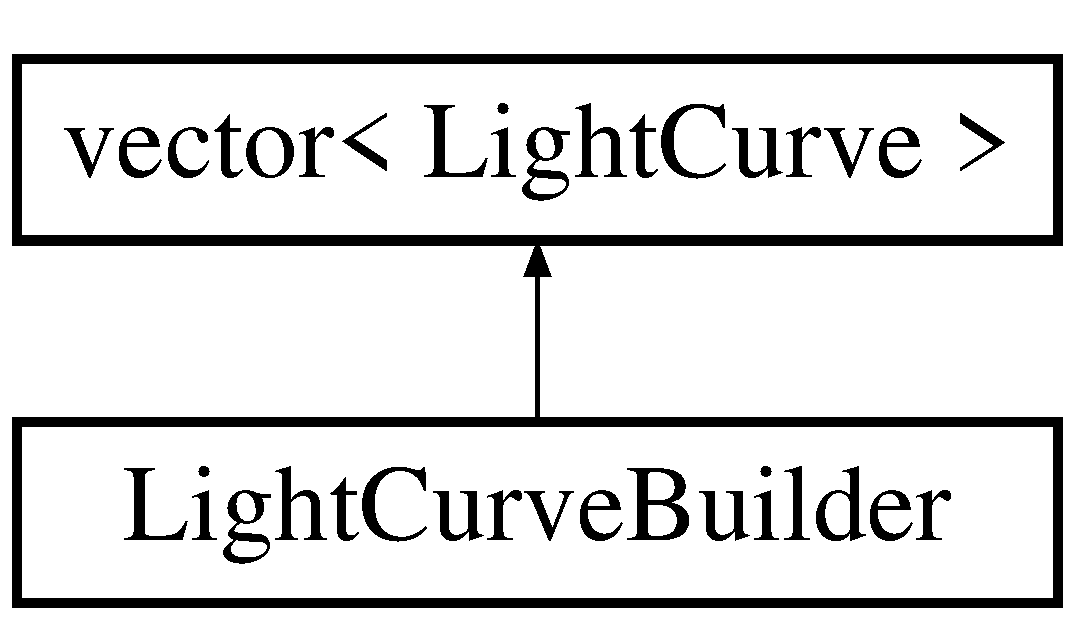
\includegraphics[height=2cm]{class_lightcurvebuilder}
\end{center}
\end{figure}
\subsubsection*{Public Methods}
\begin{CompactItemize}
\item 
\index{LightCurveBuilder@{LightCurveBuilder}!LightCurveBuilder@{Light\-Curve\-Builder}}\index{LightCurveBuilder@{LightCurveBuilder}!LightCurveBuilder@{Light\-Curve\-Builder}}
{\bf Light\-Curve\-Builder} (const Reduced\-Image\-List \&Images)\label{class_lightcurvebuilder_a0}

\begin{CompactList}\small\item\em main constructor.\item\end{CompactList}\item 
\index{LightCurveBuilder@{LightCurveBuilder}!LightCurveBuilder@{Light\-Curve\-Builder}}\index{LightCurveBuilder@{LightCurveBuilder}!LightCurveBuilder@{Light\-Curve\-Builder}}
{\bf Light\-Curve\-Builder} ()\label{class_lightcurvebuilder_a1}

\item 
\index{LightCurveBuilder@{LightCurveBuilder}!LightCurveBuilder@{Light\-Curve\-Builder}}\index{LightCurveBuilder@{LightCurveBuilder}!LightCurveBuilder@{Light\-Curve\-Builder}}
{\bf Light\-Curve\-Builder} (const Light\-Curve\-Builder \&Other)\label{class_lightcurvebuilder_a2}

\begin{CompactList}\small\item\em copy constructor.\item\end{CompactList}\item 
\index{operator=@{operator=}!LightCurveBuilder@{Light\-Curve\-Builder}}\index{LightCurveBuilder@{LightCurveBuilder}!operator=@{operator=}}
Light\-Curve\-Builder\& {\bf operator=} (const Light\-Curve\-Builder \&Right)\label{class_lightcurvebuilder_a3}

\item 
\index{~LightCurveBuilder@{$\sim$LightCurveBuilder}!LightCurveBuilder@{Light\-Curve\-Builder}}\index{LightCurveBuilder@{LightCurveBuilder}!~LightCurveBuilder@{$\sim$Light\-Curve\-Builder}}
{\bf $\sim$Light\-Curve\-Builder} ()\label{class_lightcurvebuilder_a4}

\item 
\index{Calibrate@{Calibrate}!LightCurveBuilder@{Light\-Curve\-Builder}}\index{LightCurveBuilder@{LightCurveBuilder}!Calibrate@{Calibrate}}
void {\bf Calibrate} (const double \&Nfwhm) const\label{class_lightcurvebuilder_a5}

\begin{CompactList}\small\item\em should calibrate properly the lightcurve, but does not.\item\end{CompactList}\item 
\index{Init@{Init}!LightCurveBuilder@{Light\-Curve\-Builder}}\index{LightCurveBuilder@{LightCurveBuilder}!Init@{Init}}
bool {\bf Init} (const vector$<$ {\bf Point} $>$ \&SNe)\label{class_lightcurvebuilder_a6}

\begin{CompactList}\small\item\em init the lightcurve.\item\end{CompactList}\item 
\index{Init@{Init}!LightCurveBuilder@{Light\-Curve\-Builder}}\index{LightCurveBuilder@{LightCurveBuilder}!Init@{Init}}
bool {\bf Init} (const vector$<$ {\bf Point} $>$ \&SNe, const string \&catalogue)\label{class_lightcurvebuilder_a7}

\begin{CompactList}\small\item\em init the lightcurve with a catalogue of standard stars.\item\end{CompactList}\item 
\index{InitFiducials@{InitFiducials}!LightCurveBuilder@{Light\-Curve\-Builder}}\index{LightCurveBuilder@{LightCurveBuilder}!InitFiducials@{Init\-Fiducials}}
void {\bf Init\-Fiducials} (const Base\-Star\-List \&Fid\-List)\label{class_lightcurvebuilder_a8}

\begin{CompactList}\small\item\em init all common objects.\item\end{CompactList}\item 
\index{StarListPhotometry@{StarListPhotometry}!LightCurveBuilder@{Light\-Curve\-Builder}}\index{LightCurveBuilder@{LightCurveBuilder}!StarListPhotometry@{Star\-List\-Photometry}}
void {\bf Star\-List\-Photometry} ()\label{class_lightcurvebuilder_a9}

\begin{CompactList}\small\item\em performs a quick photometry from the starlists.\item\end{CompactList}\item 
\index{SubAperPhotometry@{SubAperPhotometry}!LightCurveBuilder@{Light\-Curve\-Builder}}\index{LightCurveBuilder@{LightCurveBuilder}!SubAperPhotometry@{Sub\-Aper\-Photometry}}
void {\bf Sub\-Aper\-Photometry} (const double \&Nfwhm)\label{class_lightcurvebuilder_a10}

\begin{CompactList}\small\item\em performs aperture photometry on the subtractions.\item\end{CompactList}\item 
\index{BuildKernelsAndSubs@{BuildKernelsAndSubs}!LightCurveBuilder@{Light\-Curve\-Builder}}\index{LightCurveBuilder@{LightCurveBuilder}!BuildKernelsAndSubs@{Build\-Kernels\-And\-Subs}}
void {\bf Build\-Kernels\-And\-Subs} ()\label{class_lightcurvebuilder_a11}

\begin{CompactList}\small\item\em build the kernels among the reference and the other images.\item\end{CompactList}\item 
\index{SimFitPhotometry@{SimFitPhotometry}!LightCurveBuilder@{Light\-Curve\-Builder}}\index{LightCurveBuilder@{LightCurveBuilder}!SimFitPhotometry@{Sim\-Fit\-Photometry}}
void {\bf Sim\-Fit\-Photometry} ()\label{class_lightcurvebuilder_a12}

\begin{CompactList}\small\item\em performs simultaneous photometry for each lightcurve star.\item\end{CompactList}\item 
\index{write@{write}!LightCurveBuilder@{Light\-Curve\-Builder}}\index{LightCurveBuilder@{LightCurveBuilder}!write@{write}}
void {\bf write} (const string \&Middle\-Name) const\label{class_lightcurvebuilder_a13}

\begin{CompactList}\small\item\em write something.\item\end{CompactList}\end{CompactItemize}
\subsubsection*{Public Attributes}
\begin{CompactItemize}
\item 
\index{Reference@{Reference}!LightCurveBuilder@{Light\-Curve\-Builder}}\index{LightCurveBuilder@{LightCurveBuilder}!Reference@{Reference}}
{\bf Night}$\ast$ {\bf Reference}\label{class_lightcurvebuilder_m0}

\begin{CompactList}\small\item\em a pointer to the reference night.\item\end{CompactList}\item 
\index{Nights@{Nights}!LightCurveBuilder@{Light\-Curve\-Builder}}\index{LightCurveBuilder@{LightCurveBuilder}!Nights@{Nights}}
Night\-List {\bf Nights}\label{class_lightcurvebuilder_m1}

\begin{CompactList}\small\item\em the list of images where each lightcurve point is refered.\item\end{CompactList}\item 
\index{BandName@{BandName}!LightCurveBuilder@{Light\-Curve\-Builder}}\index{LightCurveBuilder@{LightCurveBuilder}!BandName@{Band\-Name}}
string {\bf Band\-Name}\label{class_lightcurvebuilder_m2}

\begin{CompactList}\small\item\em a band name associated with this list.\item\end{CompactList}\item 
\index{nsn@{nsn}!LightCurveBuilder@{Light\-Curve\-Builder}}\index{LightCurveBuilder@{LightCurveBuilder}!nsn@{nsn}}
unsigned {\bf nsn}\label{class_lightcurvebuilder_m3}

\begin{CompactList}\small\item\em the number of supernovae.\item\end{CompactList}\end{CompactItemize}


\subsubsection{Detailed Description}
Lightcurve builder for one band. Execute different types of photometry.



The documentation for this class was generated from the following file:\begin{CompactItemize}
\item 
{\bf lightcurvebuilder.h}\end{CompactItemize}
